\begin{figure*}[ht!]
    \centering
    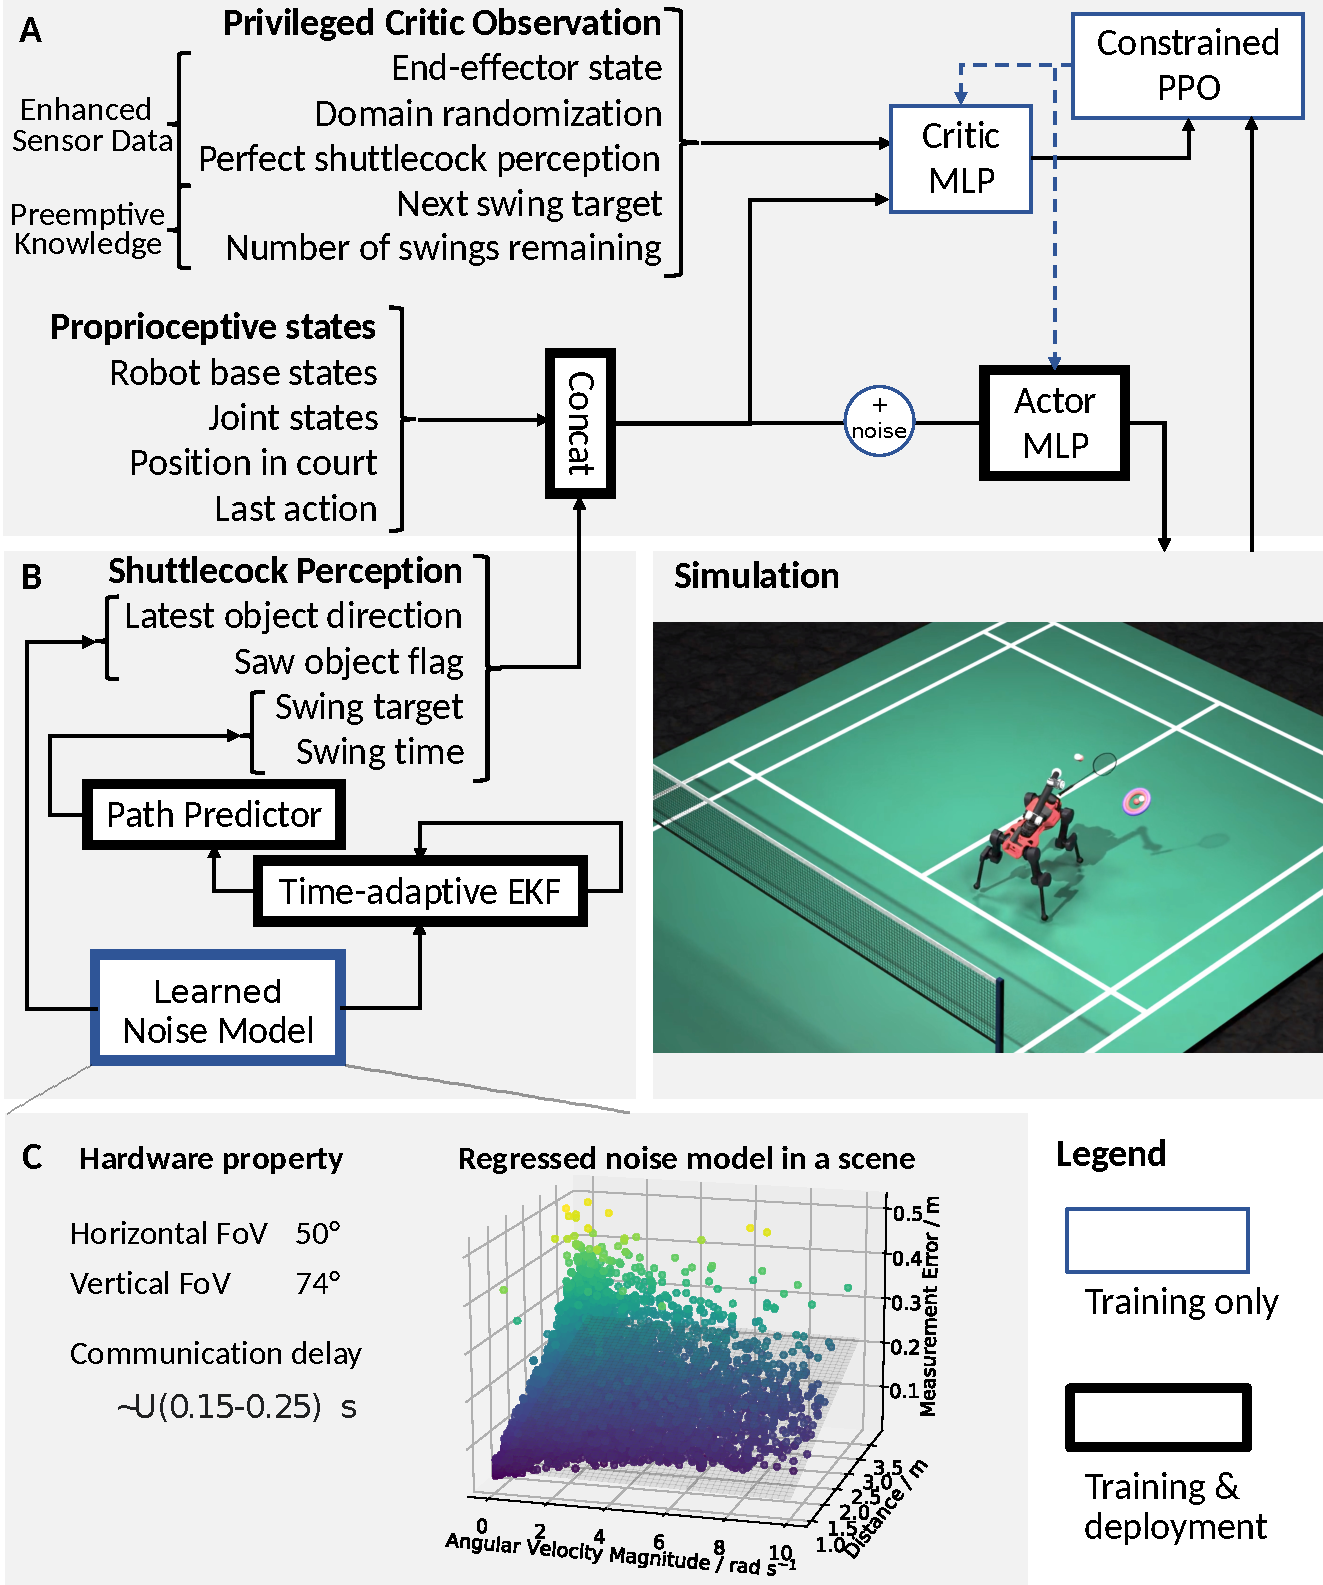
\includegraphics[width=0.8\textwidth]{Figures/TrainingPipeline/training_pipeline_vertical.pdf}
    \caption{\textbf{Overview of the training method. (A)} Joint control policy training with RL. The policy is trained with an asymmetric actor-critic, with privileged environment states and MDP information given only to the critic network. The policy receives the noised proprioceptive states and shuttlecock perception with simulated noise. \textbf{(B)} The shuttlecock perception module in simulation. The time-adaptive EKF and the path predictor are reused during the deployment. During the training, we used a regressed perception noise model based on real camera noise collected from the hardware. \textbf{(C)} Object perception noise model. The object is in the simulation with the regressed detection probability and measurement noise if it is in the camera FOV.}
    \label{fig:training_pipeline}
\end{figure*}